\documentclass[10pt,a4paper]{article}
\usepackage[utf8]{inputenc}
\usepackage[T1]{fontenc}
\usepackage[french]{babel}
\usepackage{booktabs,graphicx,geometry,hyperref,xcolor,amsmath,amssymb,array}
\usepackage{pdflscape,longtable,float,caption,titlesec}
\geometry{margin=1.6cm}
\usepackage{url}\urlstyle{tt}
\hypersetup{colorlinks=true,linkcolor=blue!45!black,citecolor=blue!45!black}
\captionsetup{font=small,labelfont=bf}
% Densité : on laisse LaTeX placer les flottants (pas de [H] figé)
\setcounter{topnumber}{3}\setcounter{bottomnumber}{2}
\setcounter{totalnumber}{5}
\renewcommand{\topfraction}{0.92}
\renewcommand{\bottomfraction}{0.75}
\renewcommand{\textfraction}{0.06}
\renewcommand{\floatpagefraction}{0.75}
\setlength{\parskip}{3pt}

\titleformat{\section}{\large\bfseries}{\thesection}{0.8em}{}
\renewcommand{\arraystretch}{1.05}

\title{\huge\textbf{Compendium de données}\\[4pt]
\large Arctic-TVC — benchmark de modèles de fondation visuels pour la\\
classification de végétation arctique par drone\\[6pt]
\normalsize Toutes les données du dépôt, en tableaux et figures}
%\author{Mémoire M.Sc. en informatique — UQAM\\
%Co-direction : M. Bouguessa (méthodologie ML), E. Laliberté (écologie)}
\date{\today}

\begin{document}
\maketitle

\begin{abstract}
\noindent Ce document rassemble, sous une forme unique et vérifiable, l'ensemble des
mesures produites par le projet : 42~modèles évalués par probe linéaire canonique
(LogisticRegression lbfgs multinomial, grille $C\in[10^{-4},10]$, \texttt{best\_C}
par validation, BLAS mono-thread), 189~runs d'affinage (courbes de données,
ablations LoRA, distillation spatiale) et 24~runs de probing gelé, 21~métriques de
géométrie latente recalculées sous un protocole homogène (par seed, à $n$ fixe),
tests de significativité par bootstrap apparié hiérarchique sur le palier
compétitif (35~modèles, 595~paires théoriques, 528 testées), transférabilité
(LogME, $k$-NN), et régime few-shot. Il ne propose pas d'interprétation : chaque
tableau porte sa source, chaque figure sa légende, et l'annexe~D donne le fichier
et le script qui produisent chaque famille de chiffres.

\vspace{6pt}
\noindent\textbf{Résultat central.} L'adaptation paramétrique d'un backbone fonctionne
— LoRA r=8 bat son propre backbone gelé de +0,0114 ($p=0{,}0012$, rejeté par
Benjamini-Hochberg), et sur SimDINOv2-B les bras b911/b611/NormTuning battent le
leur ($p\leq0{,}0043$) — mais aucun modèle \emph{déployable} (tuile seule) ne
dépasse significativement le meilleur gelé : LoRA r=8 contre DINOv3-L donne
$\Delta=+0{,}0038$, $p=0{,}39$. Seule la borne fusionnée R2 (contexte requis à
l'inférence, non déployable) dépasse tout le monde ($+0{,}025$ à $+0{,}029$,
$p<10^{-4}$). Sur SimDINOv2-B, le paysage de l'adaptation est \emph{plat} :
13~bras LoRA/PEFT (rang 2 à 32, scaling 1 à 4, blocs hauts/bas, Q+K+V, rsLoRA)
tiennent dans 0,0067 de F1, et NormTuning (normes + tête, $\approx$47k paramètres)
égale LoRA au millième près. Le vrai levier, c'est l'information, pas les poids :
le voisinage spatial de la tuile (contexte 512--1024px) apporte +0,025 à +0,034 de
F1, et un pré-entraînement aligné au domaine (iNat-Plantae) décode ce voisinage
mieux, gelé, que DINOv3 entraîné. Avec un palier élargi à 35~modèles, la famille
séparabilité (Fisher, silhouette, NC1, Calinski-Harabasz, Davies-Bouldin) ordonne
les modèles significativement mieux que le hasard (64 à 69~\% des paires,
$p_{BH}\leq0{,}046$) ; la famille spectrale reste anti-prédictive (41--42~\%),
confirmant que sa corrélation d'ensemble est portée par les modèles cassés.

\vspace{6pt}
\noindent\textbf{Précautions de lecture} : (i)~trois définitions distinctes du
« rang effectif » ont circulé sous le même nom, avec un écart d'un facteur~7
(§\ref{sec:geom}) ; (ii)~la géométrie mesurée sur le jeu d'entraînement confond
richesse de la représentation et taille d'échantillon, puisque le rang est borné
par $\min(n,D)$ (§\ref{sec:curves}) ; (iii)~plusieurs pipelines de courbe de
données coexistent dans le dépôt et donnent, pour le même régime à 100\,\% des
données, des F1 séparés de 0,024 (§\ref{sec:curves}) ; (iv)~deux conventions de
probe coexistent (canonique contre interne des runs) et leurs notes de tableau
annoncent l'écart mesuré plutôt que de le laisser deviner (§\ref{sec:signif}) ;
(v)~la courbe de données couvre \textbf{deux backbones différents} — LoRA r=8 part
de DINOv3-B, les trois autres régimes d'un ViT-B/16 ImageNet — et les deux familles
sont présentées séparément partout dans ce document.
\end{abstract}

\tableofcontents
\newpage

% ════════════════════════════════════════════════════════════
\section{Jeu de données et protocole}\label{sec:data}
% ════════════════════════════════════════════════════════════

\input{tables/t_dataset}

\input{tables/t_support}

\begin{figure}[htbp]
\centering
\includegraphics[width=0.78\textwidth]{figs/perf_support_vs_f1.png}
\caption{F1 d'une classe en fonction de son support dans le jeu test. Un point par
modèle du palier (35), le trait horizontal est la moyenne. Le seuil d'apprenabilité
se situe autour de 200~tuiles de test : en dessous, aucun modèle n'obtient un F1
non nul.}
\end{figure}

\input{tables/t_pipelines}

% ════════════════════════════════════════════════════════════
\section{Performances — 42 modèles}\label{sec:perf}
% ════════════════════════════════════════════════════════════

Le tableau maître compte 42~modèles : 11~gelés, 29~affinés à 3~seeds (LoRA, Full,
MHSA, NormTuning, distillation spatiale) et 2~bornes fusionnées non déployables
(Contexte R2 et SimDINOv2-B entraînés, contexte requis à l'inférence). Les 13~bras
de l'ablation SimDINOv2-B (Stage~A, §\ref{sec:peft}) y figurent avec leur F1
canonique (reprobe mono-thread sur les mêmes embeddings et le même test que le
benchmark) ; leurs best\_C et époques viennent du probe interne des runs.

\begin{landscape}
\small
\input{tables/t_master}
\end{landscape}

\begin{figure}[htbp]
\centering
\includegraphics[width=0.90\textwidth]{figs/perf_ranking_ci.png}
\caption{Classement par F1-macro (11~classes présentes), probe linéaire canonique.
Barre = $\pm\sigma$ inter-seed ; traits verticaux = seeds individuels. Le palier
compétitif (35~modèles, de 0,5080 à 0,4689) contient un décrochage de tête interne
(+0,016 entre les deux bornes fusionnées SimDINOv2-B et R1) : ce sont des designs
non déployables, pas la fin du bloc. La rupture qui borne le palier vaut +0,0069,
soit environ quatre fois l'écart médian entre rangs consécutifs.}
\end{figure}

\subsection{DINOv3-B gelé contre ses régimes}

\input{tables/t_dinov3b_regimes}

\subsection{SimDINOv2-B gelé contre ses régimes}

\input{tables/t_simb_regimes}

\subsection{Détail par classe}

\begin{landscape}
\input{tables/t_per_class_models}
\end{landscape}

\begin{figure}[htbp]
\centering
\includegraphics[width=0.84\textwidth]{figs/perf_per_class_heatmap.png}
\caption{F1 par classe des modèles du palier, triés par F1-macro décroissant
(probe interne des runs — même convention que le bootstrap).}
\end{figure}

\begin{figure}[htbp]
\centering
\includegraphics[width=\textwidth]{figs/perf_confusion.png}
\caption{Matrices de confusion à 100\,\% des données, normalisées par ligne
(vraie classe). Probe canonique réajusté sur les embeddings train du modèle avec son
\texttt{best\_C}.}
\end{figure}

\subsection{Effet du schéma de classes}

\begin{figure}[htbp]
\centering
\includegraphics[width=0.92\textwidth]{figs/perf_schemas.png}
\caption{Le même modèle sous les schémas 12, 11 et 8~classes.}
\end{figure}

\input{tables/t_schemas}

% ════════════════════════════════════════════════════════════
\section{Courbes de données}\label{sec:curves}
% ════════════════════════════════════════════════════════════

Les runs d'affinage des courbes (plus les 24~runs de probing gelé) forment
\textbf{deux expériences distinctes} : Full et MHSA affinent un ViT-B/16
ImageNet-1k (Scratch = même architecture sans pré-entraînement, référence gelée
ViT-B/16 IN-1k $=0{,}4500$) ; LoRA r=8 adapte DINOv3 ViT-B/16 LVD (référence gelée
$=0{,}4712$). Une courbe de la première famille et une de la seconde ne se
comparent pas point à point — l'écart mélangerait l'effet du régime d'adaptation
et celui du pré-entraînement, qui vaut déjà +0,021 avant tout affinage. Figures :
un panneau par famille, ou trait plein (DINOv3-B) contre tireté (ImageNet) et
pointillé (sans pré-entraînement). Tableaux : colonnes groupées par backbone.

\begin{figure}[htbp]
\centering
\includegraphics[width=\textwidth]{figs/dc_curves_by_init.png}
\caption{Un panneau par backbone de départ, échelle des ordonnées commune. Chaque
famille porte sa propre référence gelée (ligne grise = backbone évalué sur 100\,\% des
données, sans affinage). Bandes = $\pm\sigma$ sur 3~seeds.}
\end{figure}

\input{tables/t_dc_11cls}

\input{tables/t_thresholds}

\input{tables/t_frozen_probe}

\begin{figure}[htbp]
\centering
\includegraphics[width=\textwidth]{figs/dc_accuracy_epoch.png}
\caption{Exactitude globale et époque du meilleur checkpoint. La convergence est 2 à
3~fois plus rapide à 100\,\% des données qu'à 1\,\%.}
\end{figure}

\subsection{Courbe spatiale : le volume ne suffit pas, la couverture compte}

Le tirage aléatoire par tuiles surestime la transférabilité : à volume égal, une
courbe contrôlée par blocs spatiaux contigus (puis par orthomosaïques entières)
plafonne plus tard et plus bas. Le plateau de la courbe aléatoire ($\approx$5\,\%
du volume) est un artefact d'autocorrélation spatiale ; le plateau spatial se situe
entre 50 et 75\,\% du volume.

\begin{figure}[htbp]
\centering
\includegraphics[width=0.85\textwidth]{figs/figs_spatial_structure.png}
\caption{Blocs spatiaux contigus (fractions $<$25\,\%) puis orthomosaïques entières
($\geq$25\,\%).}
\end{figure}

\input{tables/t_spatial_results}

\begin{figure}[htbp]
\centering
\includegraphics[width=0.85\textwidth]{figs/fig_spatial_vs_random_11cls.png}
\caption{Courbe spatiale contre courbe aléatoire (LoRA r=8 DINOv3-B). Le tirage
aléatoire surestime jusqu'à +0,33~point à 1\,\%.}
\end{figure}

\subsection{Par classe}

\begin{figure}[htbp]
\centering
\includegraphics[width=\textwidth]{figs/dc_per_class_heatmap.png}
\caption{F1 de chaque classe à chaque fraction, une planche par régime.}
\end{figure}

\begin{figure}[htbp]
\centering
\includegraphics[width=\textwidth]{figs/dc_per_class_curves.png}
\caption{Les 8~classes évaluables, une par panneau, 4~régimes superposés.}
\end{figure}

\input{tables/t_per_class_lora}

\subsection{Régime few-shot}

\begin{figure}[htbp]
\centering
\includegraphics[width=0.84\textwidth]{figs/dc_fewshot.png}
\caption{Probing linéaire sur modèles gelés, de 5 à 1\,000~tuiles annotées par classe.
Couleur = famille de pré-entraînement ; style de trait = taille du backbone.}
\end{figure}

\input{tables/t_fewshot}

\subsection{Géométrie en fonction du volume, à $n$ fixe}

\begin{figure}[htbp]
\centering
\includegraphics[width=\textwidth]{figs/dc_geometry_multipanel.png}
\caption{Douze métriques géométriques en fonction du volume d'entraînement, toutes
calculées sur le jeu test ($n=17\,598$ pour tous les points).}
\end{figure}

\begin{figure}[htbp]
\centering
\includegraphics[width=\textwidth]{figs/dc_rankme_n_control.png}
\caption{Contrôle du biais de taille d'échantillon. À gauche, le rang effectif mesuré
sur le train suit la borne $\min(n,D)$ tant que $n<D$. À droite, à $n$ fixe, la
tendance disparaît pour les régimes pré-entraînés.}
\end{figure}

\input{tables/t_geometry_datacurve}

% ════════════════════════════════════════════════════════════
\section{Adaptation paramétrique : ablations LoRA et PEFT}\label{sec:peft}
% ════════════════════════════════════════════════════════════

\subsection{DINOv3-B : rang et position}

L'ablation du rang (r $\in\{2,4,8,16,32\}$, $\alpha=2r$, 3~seeds) montre un plateau
r=2/4/8 puis une décroissance à r=16/32 : le rang 8 du manuscrit est sur le plateau,
pas à un optimum fragile. L'ablation de position (même budget, 147k paramètres)
montre que le bénéfice vient des blocs profonds : adapter les 6~blocs hauts
(6--11) égale le LoRA complet à 12~blocs, adapter les 6~blocs bas retombe au niveau
du Full FT.

\input{tables/t_lora_rank}

\begin{figure}[htbp]
\centering
\includegraphics[width=0.9\textwidth]{figs/lora_rank_curve.png}
\caption{F1 en fonction du rang LoRA (DINOv3-B). Plateau puis décroissance.}
\end{figure}

\input{tables/t_lora_block_ablation}

\subsection{SimDINOv2-B : le palier plat (Stage A, 13 bras)}

Transposition à SimDINOv2-B de la question « meilleur LoRA » : 13~bras $\times$
3~seeds (position, rang 2 à 32, scaling 1 à 4, Q+K+V, rsLoRA, NormTuning), même
test que le benchmark, F1 canonique. \textbf{Tout le palier tient dans 0,0067} :
ni le rang, ni le scaling, ni le type ne battent l'ancre r8a8 tous blocs (0,4781)
au-delà du bruit. Trois constats structurent la lecture :

\begin{itemize}
\item \textbf{NormTuning = LoRA au millième près} (0,4783 $\pm$ 0,0004 contre
0,4781 $\pm$ 0,0028) avec $\approx$47k paramètres (normes + tête, aucun
adaptateur) : l'adaptation de SimB vaut ce que vaut sa normalisation.
\item \textbf{Le scaling dégrade partout} (r=8 : 0,4781 $\to$ 0,4760 $\to$ 0,4753 ;
r=16 : 0,4769 $\to$ 0,4749 $\to$ 0,4737) : l'hypothèse rsLoRA est infirmée sur ces
données, et le décrochage r=16/32 observé sur DINOv3 n'était pas un artefact de
scaling — c'est un effet de rang réel. Convention $\alpha=r$ validée.
\item \textbf{La position se transpose} : blocs hauts $\geq$ tous blocs $\gg$
blocs bas, comme sur DINOv3-B ; b911 (3~derniers blocs, moitié du budget de b611)
est le bras le plus stable ($\pm$0,0002).
\end{itemize}

\input{tables/t_simb_ablation}

\begin{figure}[htbp]
\centering
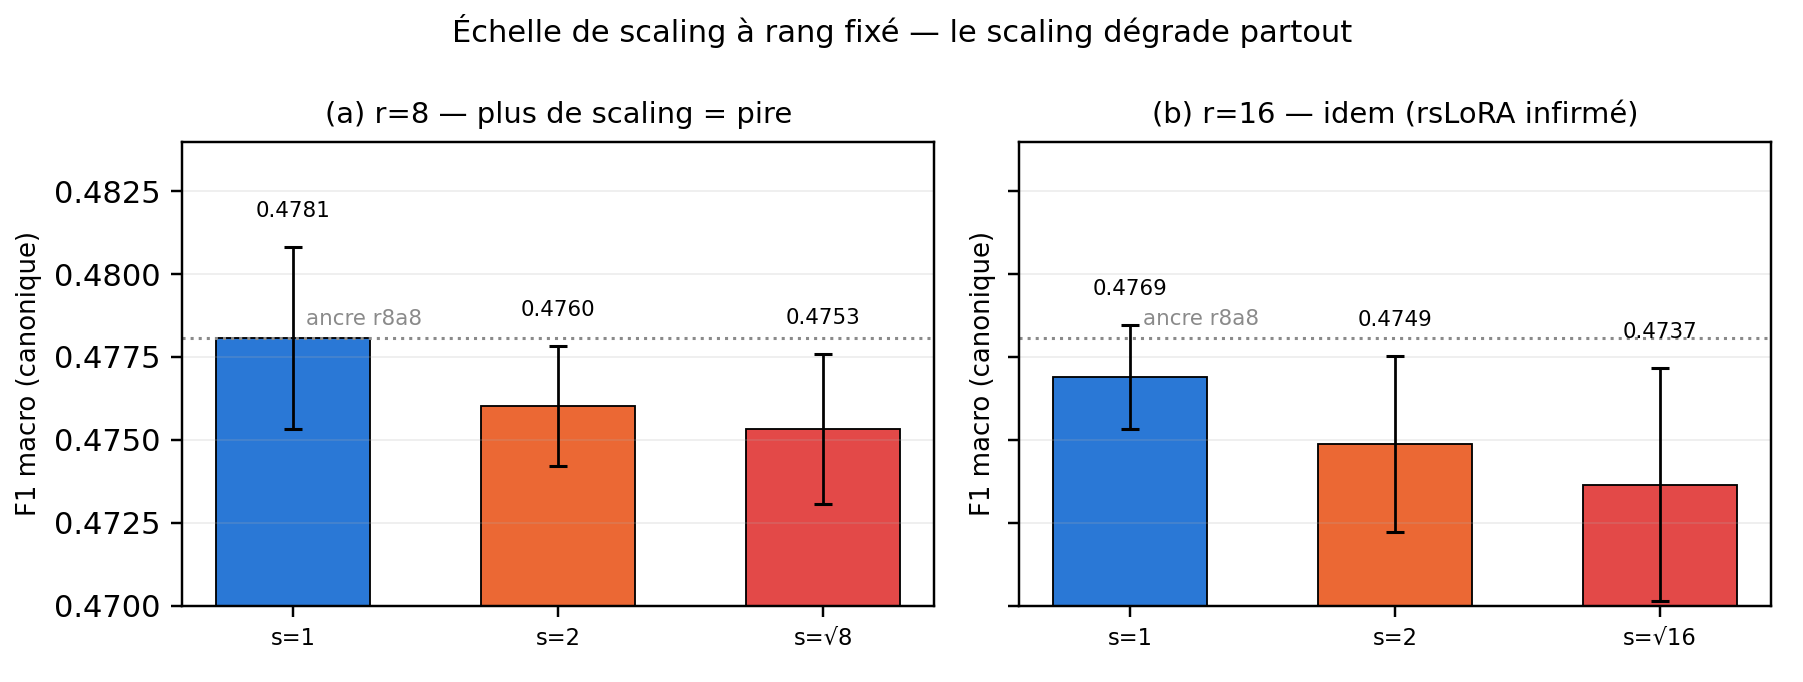
\includegraphics[width=0.92\textwidth]{figs/peft_scaling_ladder.png}
\caption{Échelle de scaling à rang fixé (r=8 et r=16) : plus de scaling = pire,
monotone. La ligne pointillée est l'ancre r8a8 tous blocs.}
\end{figure}

\begin{figure}[htbp]
\centering
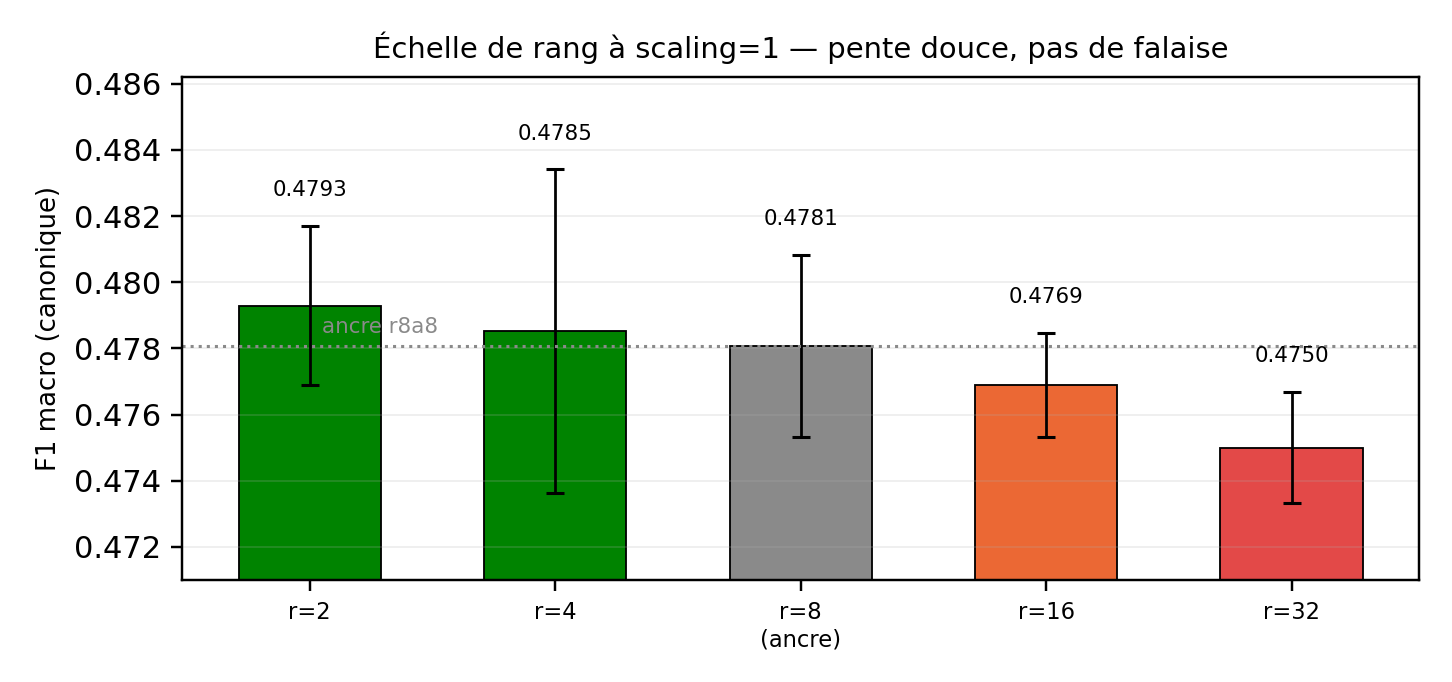
\includegraphics[width=0.72\textwidth]{figs/peft_rank_ladder.png}
\caption{Échelle de rang à scaling=1 : pente douce décroissante, pas de falaise.}
\end{figure}

\begin{figure}[htbp]
\centering
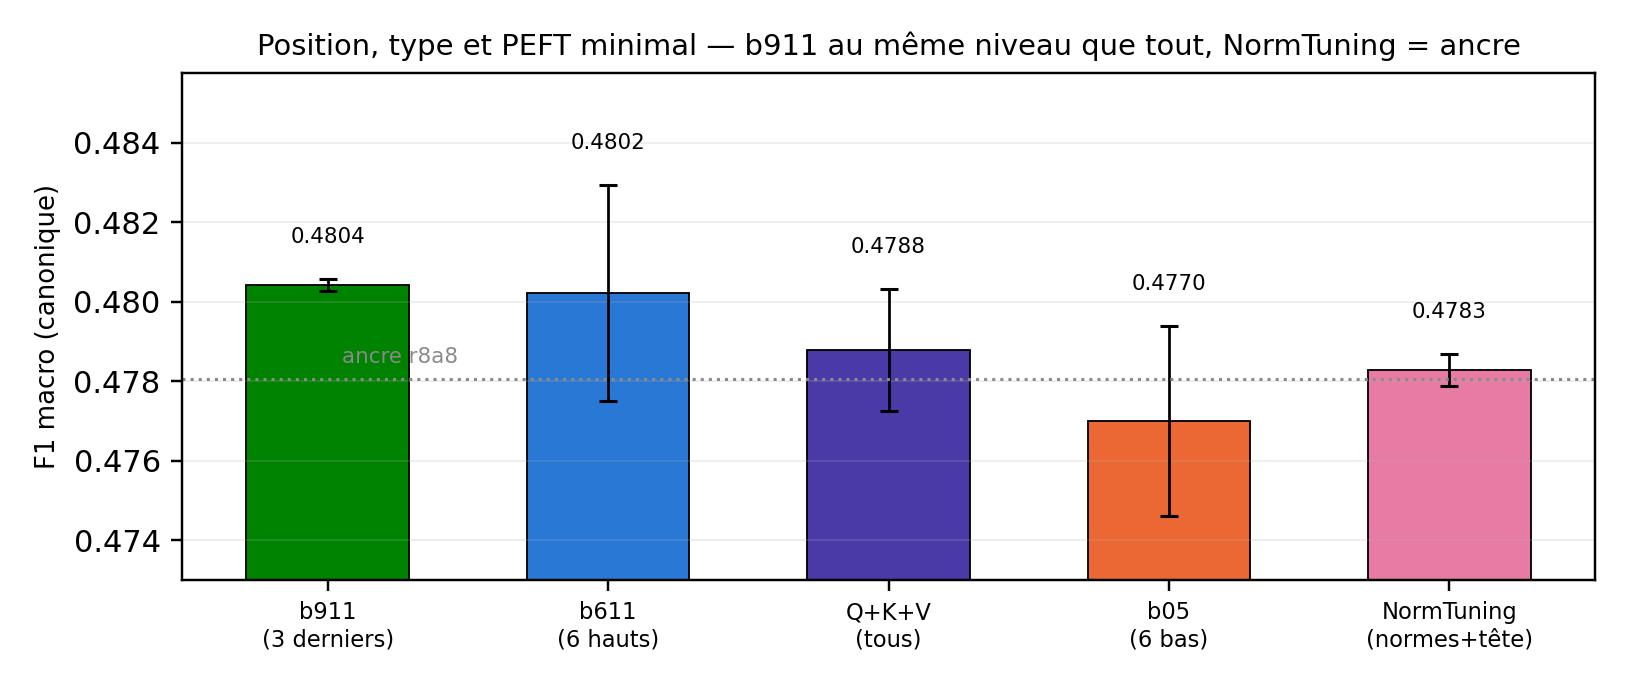
\includegraphics[width=0.80\textwidth]{figs/peft_position.png}
\caption{Position, type et PEFT minimal : b911 au niveau du LoRA complet avec un
quart du budget ; NormTuning égale l'ancre.}
\end{figure}

\noindent\textbf{Caveat de sélection du C (QKV seed2).} Le probe interne du run QKV
seed2 sélectionne $C=0{,}0001$ (F1 test 0,4873) quand le reprobe canonique
(sélection sur sous-échantillon 20k) sélectionne $C=0{,}001$ (F1 test 0,4799) : un
basculement de $C$ déplace ce seed de 0,0074. Au sommet du plateau, le choix de $C$
pèse autant que le choix du bras ; la valeur canonique est retenue, l'écart est
tracé par la table des conventions.

\subsection{Coût contre performance}

\input{tables/t_cost_perf}

\begin{figure}[htbp]
\centering
\includegraphics[width=\textwidth]{figs/cost_perf.png}
\caption{F1 contre coût (paramètres et FLOPs, échelle log). DINOv3-B + LoRA r=8
(86,3M paramètres dont 0,295M entraînables) égale ou dépasse DINOv3-H+ gelé (840M)
pour un budget d'adaptation de trois ordres de grandeur inférieur.}
\end{figure}

% ════════════════════════════════════════════════════════════
\section{Géométrie de l'espace latent}\label{sec:geom}
% ════════════════════════════════════════════════════════════

Géométrie calculée par seed puis moyennée, sur le test à $n$ fixe
(sous-échantillon 20\,000, seed~42) — jamais sur seeds concaténés (qui gonflent
l'étalement), jamais sur le train (biais de taille d'échantillon, §\ref{sec:curves}).

\input{tables/t_conventions}

\begin{figure}[htbp]
\centering
\includegraphics[width=\textwidth]{figs/geom_conventions.png}
\caption{Les deux conventions de rang effectif sont fortement corrélées entre elles
mais séparées d'un facteur 4,9 à 19,2 en valeur (médiane 7,5).}
\end{figure}

\begin{landscape}
\small
\input{tables/t_geometry_full}
\end{landscape}

\begin{figure}[htbp]
\centering
\includegraphics[width=\textwidth]{figs/geom_scatter_grid.png}
\caption{Chaque métrique face au F1 aval, tous modèles, protocole unique.}
\end{figure}

\begin{figure}[htbp]
\centering
\includegraphics[width=\textwidth]{figs/geom_spectra.png}
\caption{Spectres de covariance normalisés (log-log) et ajustement en loi de
puissance dont la pente donne $\alpha$.}
\end{figure}

\subsection{Famille DINOv3 ViT-B/16}

\input{tables/t_family}

\begin{figure}[htbp]
\centering
\includegraphics[width=\textwidth]{figs/geom_dinov3b_family.png}
\caption{Coordonnées parallèles sur la famille DINOv3-B : F1 constant à
$\pm0{,}012$, géométries nettement séparées.}
\end{figure}

\subsection{Par profondeur}

\begin{figure}[htbp]
\centering
\includegraphics[width=\textwidth]{figs/geom_layerwise.png}
\caption{Géométrie couche par couche des deux ViT-L/16 (photos vs satellite),
24~blocs, embeddings test.}
\end{figure}

\input{tables/t_layerwise}

% ════════════════════════════════════════════════════════════
\section{Transférabilité et évaluations alternatives}\label{sec:transfer}
% ════════════════════════════════════════════════════════════

\subsection{Corrélations géométrie $\leftrightarrow$ F1}

\input{tables/t_correlations}

\begin{figure}[htbp]
\centering
\includegraphics[width=0.90\textwidth]{figs/geom_corr_forest.png}
\caption{$\rho$ de Spearman et IC95 bootstrap par métrique et par population.
Points creux : IC95 traversant zéro.}
\end{figure}

\input{tables/t_kmeans_control}

\subsection{Peut-on classer les meilleurs modèles ?}

Le palier est fixé par la rupture mesurée du classement : 35~modèles de 0,5080 à
0,4689, décrochage de +0,0069 au rang suivant (environ quatre fois l'écart médian
entre rangs consécutifs). Le palier contient un décrochage de tête interne (+0,016
entre les deux bornes fusionnées SimDINOv2-B et R1) : ce sont des designs à
contexte requis à l'inférence, pas des modèles déployables — ils participent au
classement mais l'interprétation distingue les deux régimes d'usage.

Sur ce palier élargi, la famille \textbf{séparabilité de classes} (ratio de
Fisher, silhouette, Calinski-Harabasz, NC1, Davies-Bouldin) ordonne 64 à 69~\% des
paires et passe le seuil de significativité après correction BH par famille
($p\leq0{,}046$ pour Fisher, CHI, NC1, DBI ; silhouette $p=0{,}026$ en paires mais
$p=0{,}081$ en corrélation). Sa direction était stable sur tous les paliers
restreints testés (6 à 14~modèles) : l'effet existe, mais $n=14$ ne donnait pas la
puissance pour le déclarer — le verdict « artefact de petit échantillon » des
campagnes à 14~modèles était un manque de puissance, pas une absence d'effet. La
famille \textbf{spectrale} reste anti-prédictive sur le palier (41--42~\% des
paires, IC95 traversant zéro) et ne redevient positive que sur la population
complète : sa corrélation d'ensemble est portée par les modèles cassés. Seule la
pureté k-NN désigne le vrai modèle n\textsuperscript{o}~1 (R2).

\input{tables/t_tier_ranking}

\begin{figure}[htbp]
\centering
\includegraphics[width=\textwidth]{figs/geom_tier_ranking.png}
\caption{(a) Le signe dépend de la population. (b) Pouvoir d'ordonnancement sur le
palier de 35. (c) La séparabilité forme un bloc unique.}
\end{figure}

\input{tables/t_tier_signs}

\subsection{LogME}

\input{tables/t_logme}

\subsection{Probe linéaire contre $k$-NN}

\begin{figure}[htbp]
\centering
\includegraphics[width=\textwidth]{figs/perf_knn_vs_probe.png}
\caption{Probe contre $k$-NN sur les mêmes embeddings test.}
\end{figure}

\input{tables/t_knn}

% ════════════════════════════════════════════════════════════
\section{Significativité statistique}\label{sec:signif}
% ════════════════════════════════════════════════════════════

Bootstrap apparié hiérarchique (mêmes indices de tuiles et de seeds partagés entre
groupes, $n=10\,000$ rééchantillonnages, seed~42) sur les 33~groupes du palier
disposant d'embeddings test (les 2~bornes SimDINOv2-B entraînées, sans embeddings
rapatriés, restent des point-estimates documentés — toute comparaison les
impliquant ne passe pas le §4.4 d'AGENTS.md et n'est pas testée ici).

\input{tables/t_dinov3b_regimes}

\input{tables/t_simb_regimes}

\input{tables/t_ci}

% Les rejets BH en deux tableaux lisibles (1/2 contexte, 2/2 tuile seule), puis
% la version longue complète (528 paires, rejets et non-rejets).
\input{tables/t_signif_bh}

\input{tables/t_signif}

\begin{figure}[htbp]
\centering
\includegraphics[width=0.92\textwidth]{figs/perf_signif_matrix_head.png}
\caption{Matrice de significativité (a) — tête du palier (17~modèles, 136~paires
internes). La couleur porte le $\Delta$ (rouge = la ligne bat la colonne) ; les
cellules étoilées sont les paires rejetées par Benjamini-Hochberg sur les
528~paires testées.}
\end{figure}

\begin{figure}[htbp]
\centering
\includegraphics[width=0.92\textwidth]{figs/perf_signif_matrix_tail.png}
\caption{Matrice de significativité (b) — queue du palier (16~modèles). Le bloc
central sans étoile est le palier plat SimDINOv2-B : les bras d'adaptation ne se
distinguent pas l'un de l'autre.}
\end{figure}

\begin{figure}[htbp]
\centering
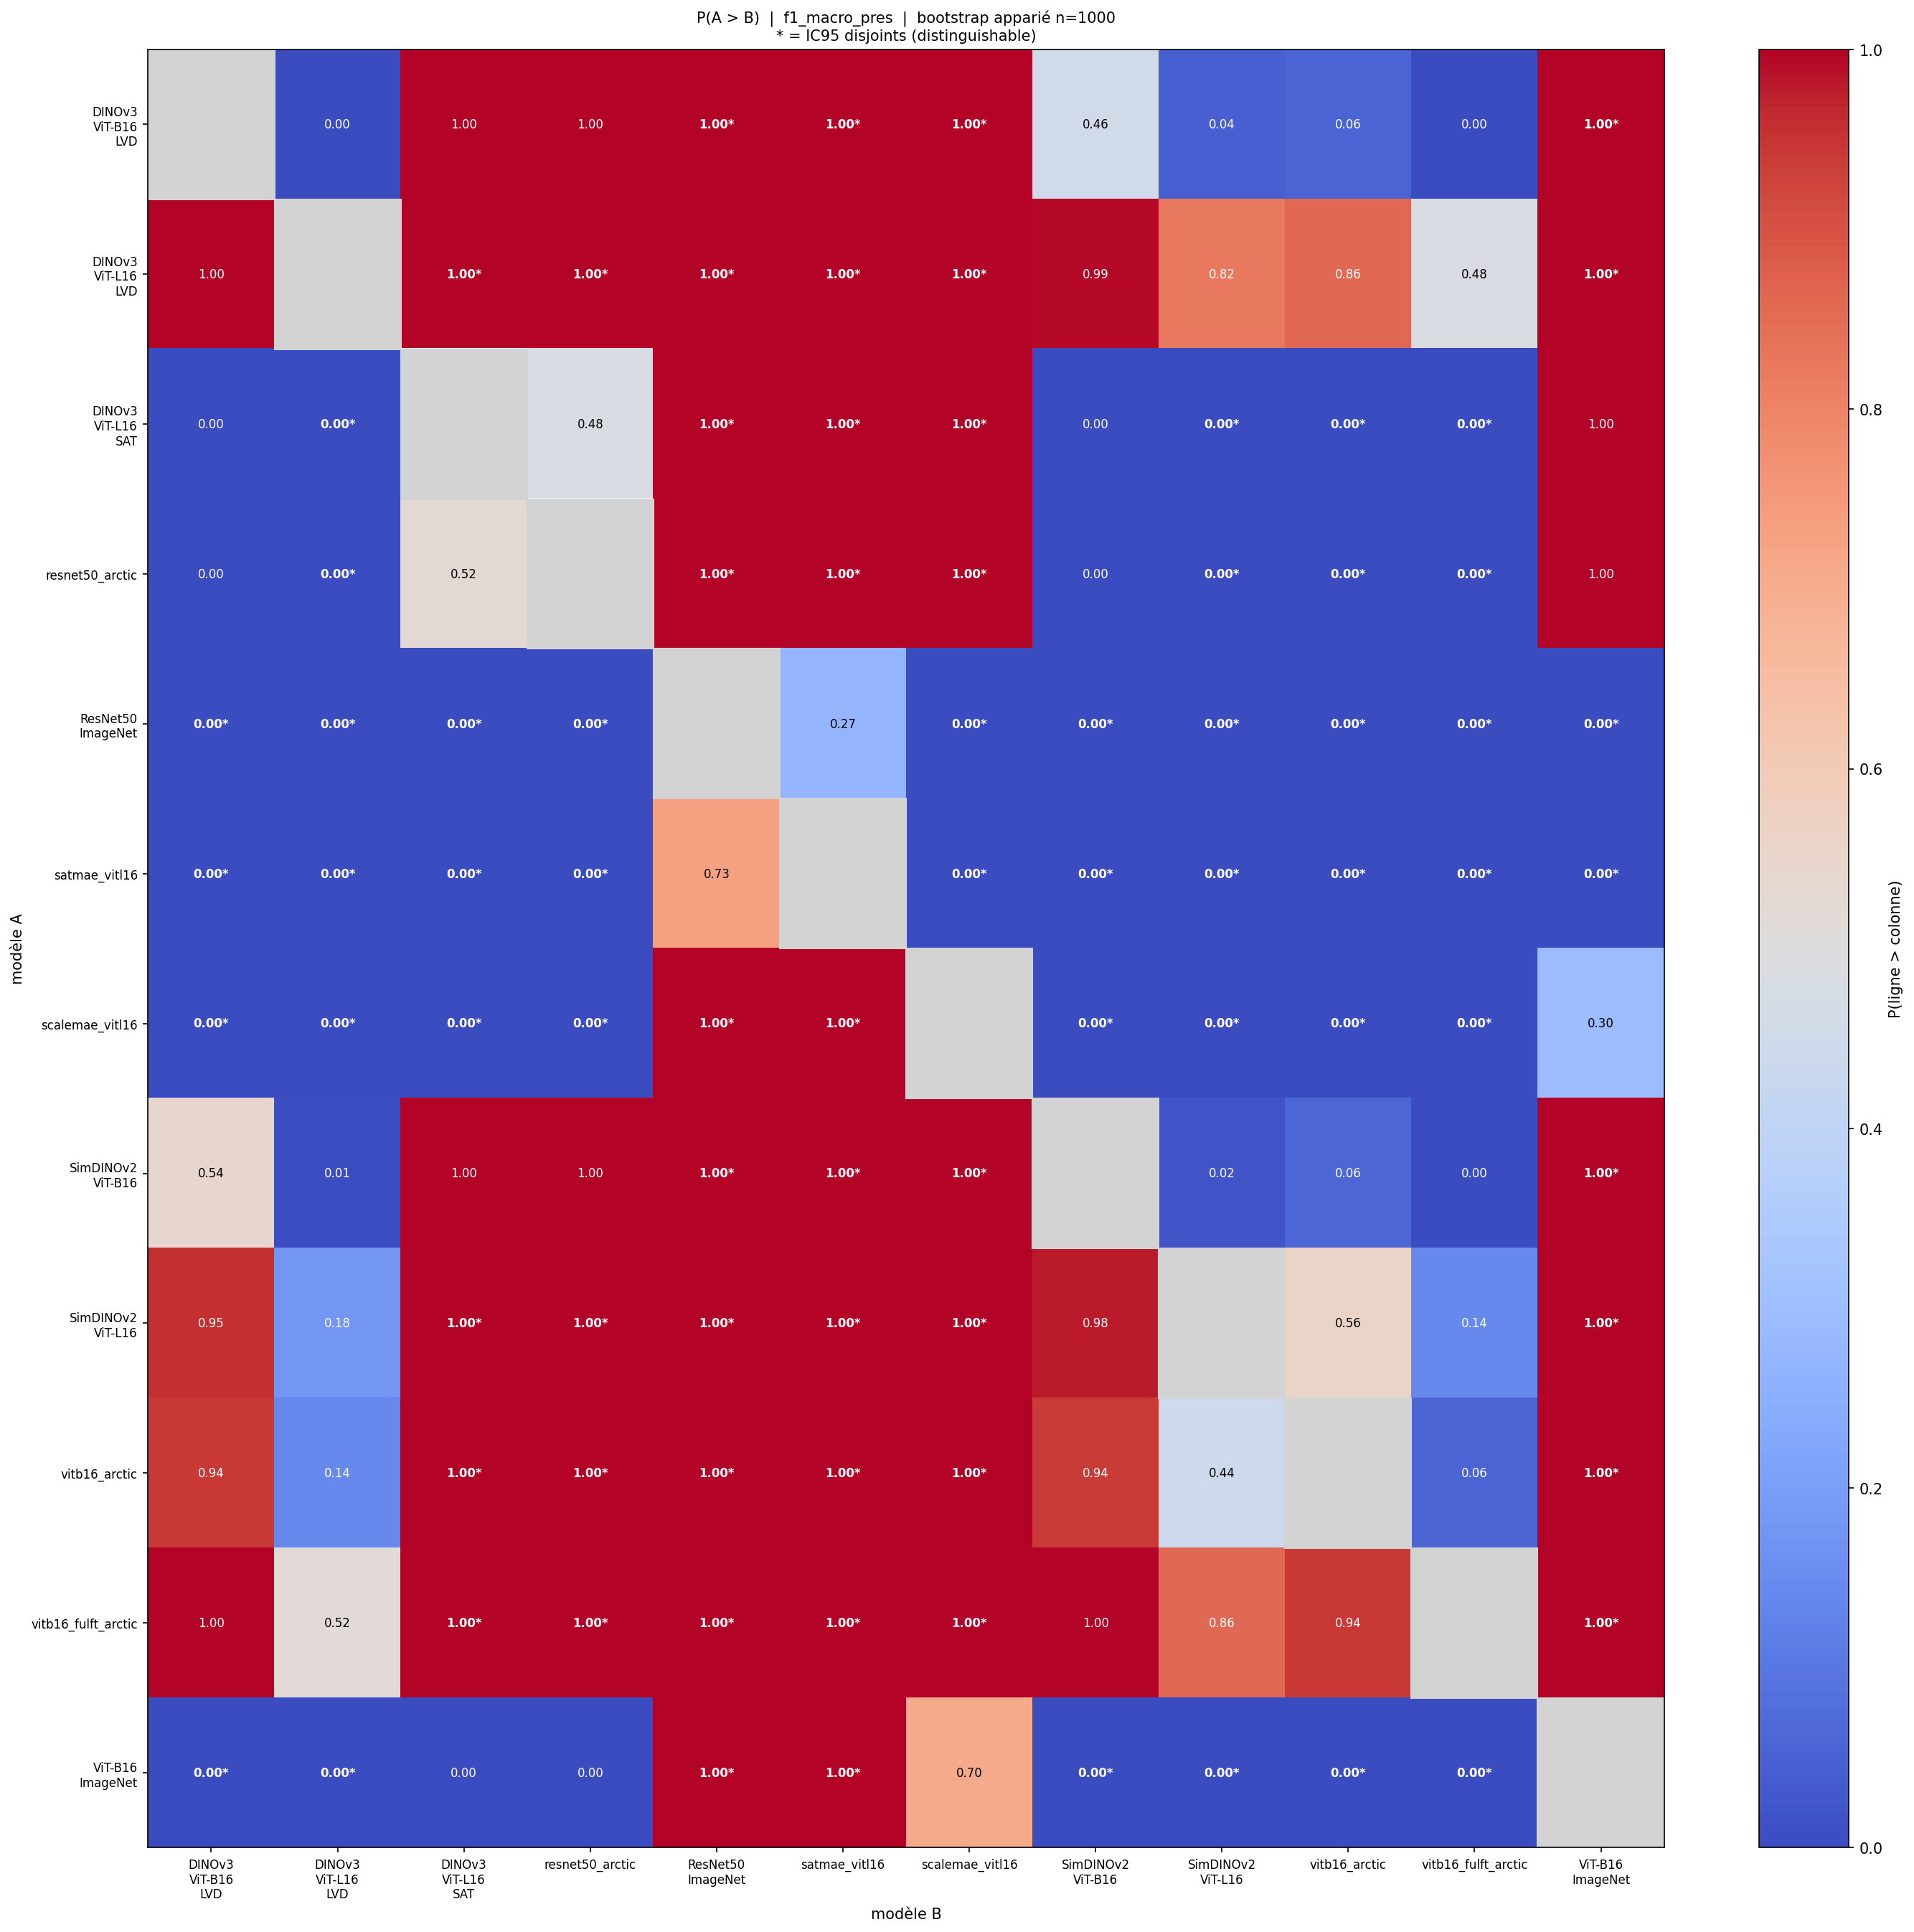
\includegraphics[width=0.72\textwidth]{../results/significance_matrix_all12.png}
\caption{Matrice de significativité — 12~modèles, campagne antérieure.}
\end{figure}

% ════════════════════════════════════════════════════════════
\section{Contexte spatial : le voisinage comme information}\label{sec:ctx}
% ════════════════════════════════════════════════════════════

Deux designs testent l'apport du contexte spatial (fenêtre centrée sur la tuile,
redimensionnée à 224) : \textbf{A} (contexte au train seulement, tuile seule à
l'inférence) et \textbf{B} (tête apprise sur [tuile;contexte], contexte requis à
l'inférence — borne supérieure théorique, non déployable). Test v3 spatial,
identique au benchmark (mêmes 17\,598~tuiles, même ordre — vérifié par hachage des
labels).

\begin{figure}[htbp]
\centering
\begin{minipage}[t]{0.49\textwidth}
\centering
\includegraphics[width=\textwidth]{figs/fig_ctx_arch_A.png}
\end{minipage}\hfill
\begin{minipage}[t]{0.49\textwidth}
\centering
\includegraphics[width=\textwidth]{figs/fig_ctx_arch_B.png}
\end{minipage}
\caption{Architectures A et B. Dans les deux cas le teacher gelé n'est utilisé
qu'au train (cible de distillation, jamais à l'inférence) : la différence de B,
c'est la tête, rien d'autre.}
\end{figure}

\input{tables/t_ctx_distill}

\begin{figure}[htbp]
\centering
\includegraphics[width=0.80\textwidth]{figs/fig_ctx_f1.png}
\caption{F1 par design (moy. 3~seeds $\pm$ std), test v3. R2 explose (+0,021 contre
R1) ; les deux SimDINOv2-B @512 entraînés plafonnent au niveau du gelé-fusionné.}
\end{figure}

\input{tables/t_ctx_matrix}

\begin{figure}[htbp]
\centering

\includegraphics[width=0.72\textwidth]{figs/fig_ctx_matrix.png}
\caption{Attribution : le contexte aide tous les modèles (+0,006 à +0,015, plafond
$\approx$0,495), mais \emph{seul} R2 (tête entraînée sur features fusionnées)
franchit 0,51 — au prix d'une tuile seule \emph{dégradée} (0,478) : le backbone
s'est \emph{spécialisé}.}
\end{figure}

\input{tables/t_ctx_controls}

\input{tables/t_ctx_sweep}

\begin{figure}[htbp]
\centering
\includegraphics[width=0.66\textwidth]{figs/fig_ctx_geom.png}
\caption{Géométrie de l'espace latent (test v3). Le fine-tuning réduit fortement
l'anisotropie (0,587 gelé $\to$ 0,33-0,45) ; la tuile seule de R2 reste plus
anisotrope (0,449) que celle de R1 (0,334) — le backbone B \emph{s'appuie sur le
contexte}. RankMe/dim constant $\Rightarrow$ \emph{pas} d'artefact de
dimensionnalité.}
\end{figure}

\noindent\textbf{Position du chapitre.} Le contexte spatial est le plus grand levier
mesuré du projet (+0,025 à +0,034), devant tout régime d'adaptation — mais à deux
conditions établies par les contrôles : appariement spatial exact (un contexte
permuté \emph{dégrade} sous la tuile seule) et exploitation apprise ou
pré-alignée (sonde sur backbone non fusionné : plafond $\approx$0,495 ; Design~B
sur DINOv3 : 0,5080 ; gelé-fusionné sur SimDINOv2-B : 0,5059 sans entraînement).

% ════════════════════════════════════════════════════════════
\section{Têtes non linéaires : la non-linéarité sauve-t-elle le contexte ?}\label{sec:heads}
% ════════════════════════════════════════════════════════════

La sonde canonique est \emph{linéaire}. Si la part d'interaction
tuile$\times$contexte était manquée par la linéarité, une tête plus riche (MLP-2,
bilinéaire-diagonale, FiLM) devrait récupérer le $+0{,}013$ qui sépare la fusion
gelée sondée ($\approx$0,495) de la fusion apprise (R2, 0,5080). Test sur (i)~les
33~groupes tuile du palier et (ii)~les 24~tags fusionnés.

\input{tables/t_head_tile}

\input{tables/t_head_fused}

\noindent\textbf{Réponse : non.} Sur la tuile seule, le MLP-2 est \emph{négatif}
contre la sonde linéaire dans 33/33~groupes ($\Delta$ moyen $-0{,}0103$) ; sur les
embeddings fusionnés, la meilleure tête non linéaire reste sous \texttt{lbfgs}
partout ($\Delta$ moyen $-0{,}0082$, 2/24~positifs). Les têtes d'interaction
elles-mêmes (\texttt{bil\_diag}, \texttt{film}) sont neutres à négatives. Le
$+0{,}013$ de R2 est donc un gain de \emph{représentation apprise}, déjà capté par
la sonde linéaire — pas une interaction que le classifieur laissait sur la table.
Corollaire méthodologique : l'écart \texttt{lbfgs}$\leftrightarrow$AdamW
($+0{,}010$ à $+0{,}013$) est un artefact d'optimiseur ; citer un $\Delta$ de tête
contre AdamW surestime l'apport de la non-linéarité.

% ════════════════════════════════════════════════════════════
\appendix
\section{Annexe A — les runs d'affinage}
% ════════════════════════════════════════════════════════════

\begin{landscape}
\footnotesize
\input{tables/t_runs_raw}
\end{landscape}

% ════════════════════════════════════════════════════════════
\section{Annexe B — F1 par classe et par fraction}
% ════════════════════════════════════════════════════════════

\input{tables/t_per_class_regimes}

\input{tables/t_dc_8cls}

\input{tables/t_dc_acc}

% ════════════════════════════════════════════════════════════
\section{Annexe C — figures d'origine des campagnes antérieures}
% ════════════════════════════════════════════════════════════

Conservées pour continuité ; les tableaux du corps de ce document les remplacent
lorsque le protocole a changé. Les figures des campagnes antérieures portant sur la
population complète de modèles ne sont plus reproduites : elles ont été tracées sur
une population qui n'est plus celle de ce document.

\begin{figure}[htbp]
\centering
\includegraphics[width=0.80\textwidth]{../results/datacurve_lora/geometry_all_metrics.png}
\caption{Géométrie LoRA r=8 vs fraction, mesurée sur le \emph{train} — campagne
\url{results/datacurve_lora/}. À comparer avec la version à $n$ fixe du
§\ref{sec:curves}.}
\end{figure}

% ════════════════════════════════════════════════════════════
\section{Annexe D — inventaire des sources}
% ════════════════════════════════════════════════════════════

\input{tables/t_sources}

\vspace{8pt}
\noindent\textbf{Reproduction complète :}
\begin{verbatim}
python3 scripts/rapport/probe_simb_stageA_canonical.py  # F1 canonique Stage A
python3 scripts/context_bouguessa_controls.py --workers 2  # contrôles R2
python3 scripts/rapport/aggregate_screening.py
python3 scripts/rapport/geometry_test_fixed_n.py     # ~35 min
python3 scripts/rapport/knn_and_confusion.py
python3 scripts/rapport/layerwise_geometry.py
python3 scripts/rapport/correlations.py
python3 scripts/rapport/tier_ranking.py
python3 scripts/rapport/significance_tier.py   # ~2 h, cache disque
python3 scripts/rapport/make_perclass_tier.py
python3 scripts/rapport/make_tables.py
for f in rapport_bouguessa/figs/make_*.py; do python3 "$f"; done
python3 scripts/rapport/check_consistency.py

\end{verbatim}

\end{document}
